\documentclass{beamer}
\usetheme{metropolis}
\usepackage{listings}
\usepackage{xcolor}

\title{Debugging \& Matplotlib}
\author{Jannusch Bigge}
\date{28.11.2023}

\begin{document}
\begin{frame}
    \titlepage
\end{frame}

\section{Matplotlib}

\begin{frame}{Matplotlib}
    Matplotlib is a plotting library.\\\pause
    Many different plots are possible.\\\pause
    \begin{itemize}
        \item Line plots
        \item Scatter plots
        \item Bar plots
        \item 3D plots
        \item ...
    \end{itemize}

\end{frame}

\begin{frame}{Matplotlib}
    Works great together with other libraries (e.g. numpy).\\\pause
    Allows you to customize your plots.\\

\end{frame}

\begin{frame}[fragile]{Matplotlib - HowTo}
    \begin{alertblock}{Attention}
        Matplotlib has two modes:
        
        \begin{itemize}
            \item<1-> Implicit mode
                \only<2-5>{
                    \begin{itemize}
                        \item<2-4> Global state-based interface mode
                        \item <3-4> like MATLAB
                        \item <4> not recommended (but always used on the internet)
                    \end{itemize}
                }
    
            \item<6-> Explicit mode
                \only<6->{
                    \begin{itemize}
                        \item<7-> Object-oriented (OO) interface
                        \item <8-> Build up the visualization in an instance of \textit{figure.Figure}
                        \item <9-> \textbf{Recommended to use!}
                    \end{itemize}
                }
        \end{itemize}
        
    \end{alertblock}
\end{frame}


\begin{frame}[fragile]{Matplotlib - HowTo}
    \begin{exampleblock}{Implicit mode}
    \end{exampleblock}
    \begin{lstlisting}[language=Python, backgroundcolor = \color{lightgray}]
import matplotlib.pyplot as plt
plt.plot([1, 2, 3, 4], [0, 0.5, 1, 0.2])
    \end{lstlisting}
    \pause
    \begin{exampleblock}{Explicit mode}
    \end{exampleblock}
    \begin{lstlisting}[language=Python, backgroundcolor = \color{lightgray}]
import matplotlib.pyplot as plt
fig = plt.figure()
ax = fig.subplots()
ax.plot([1, 2, 3, 4], [0, 0.5, 1, 0.2])
    \end{lstlisting}
\end{frame}


\begin{frame}{Matplotlib - Why explicit?}
    \begin{itemize}
        \item  <1-> More control over your plots
        \item  <2-> If you have to work on an old unreferenced axes 
        \item  <3-> Third party often uses explicit mode
    \end{itemize}
\end{frame}

\begin{frame}[fragile]{Matplotlib - Example}
    \begin{lstlisting}[language=Python, backgroundcolor = \color{lightgray}]
import matplotlib.pyplot as plt

fig = plt.figure()
ax = fig.subplots()
ax.plot([1, 2, 3, 4], [0, 0.5, 1, 0.2])
    \end{lstlisting}

\end{frame}

\begin{frame}{Matplotlib - Example}
    \begin{figure}
        \centering
        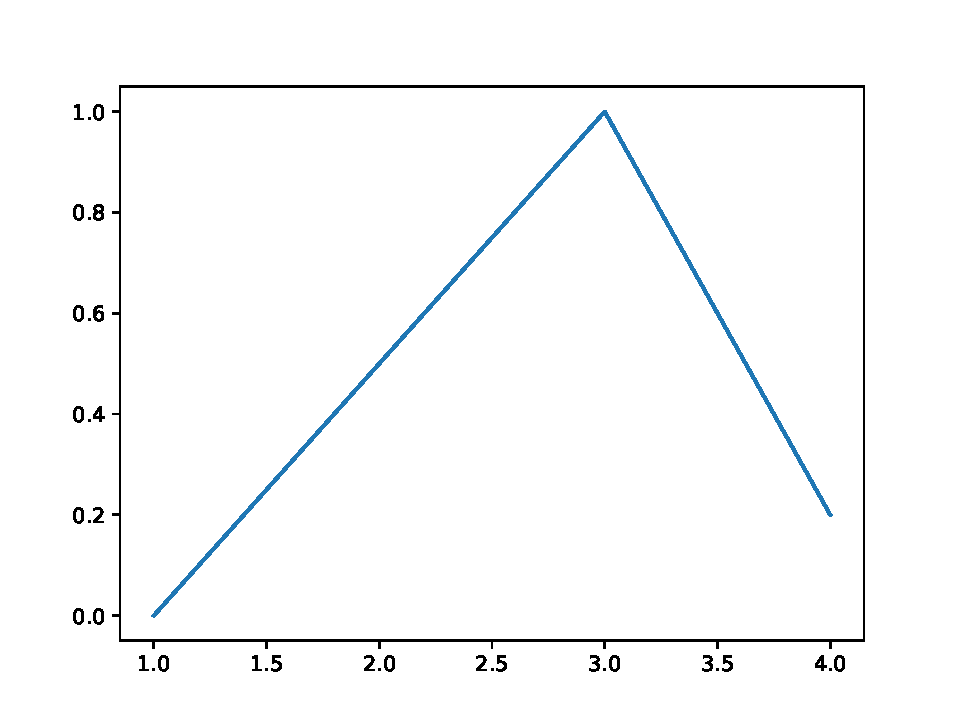
\includegraphics[width=1\textwidth]{/workspaces/python_course/slides/week_five/figures/example_1.pdf}
    \end{figure}
\end{frame}


\begin{frame}[fragile]{Matplotlib - Example}
    \begin{lstlisting}[language=Python, backgroundcolor = \color{lightgray}]
# Add some text to the figure
fig.suptitle('Explicit Interface Example')
ax.set_xlabel('x label')
ax.set_ylabel('y label')
    \end{lstlisting}

\end{frame}

\begin{frame}{Matplotlib - Example}
    \begin{figure}
        \centering
        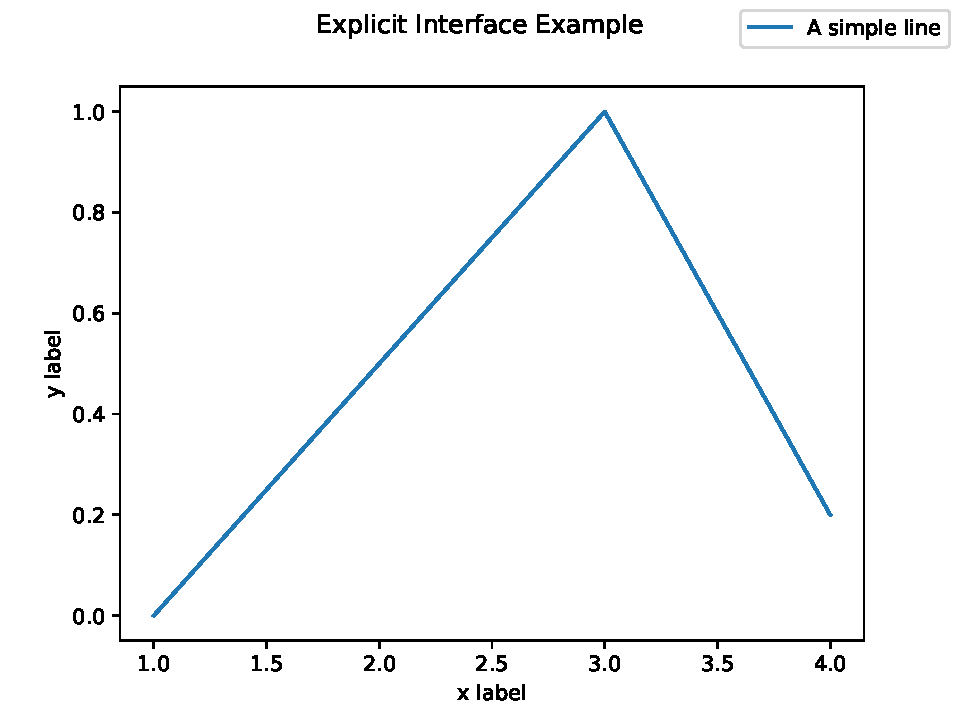
\includegraphics[width=1\textwidth]{/workspaces/python_course/slides/week_five/figures/example_2.pdf}
    \end{figure}
\end{frame}

\begin{frame}[fragile]{Matplotlib - Example}
    \begin{lstlisting}[language=Python, backgroundcolor = \color{lightgray},
        columns=fullflexible,
        breaklines=true,]
# Add another line and a second legend
ax.plot([1, 2, 3, 4], [1, 3, 1, 4], 'r--')
ax.legend(['A simple line', 'Another line'])
# And save the figure
fig.savefig("/workspaces/python_course/slides/week_five/figures/myplot.pdf")
    \end{lstlisting}

\end{frame}

\begin{frame}{Matplotlib - Example}
    \begin{figure}
        \centering
        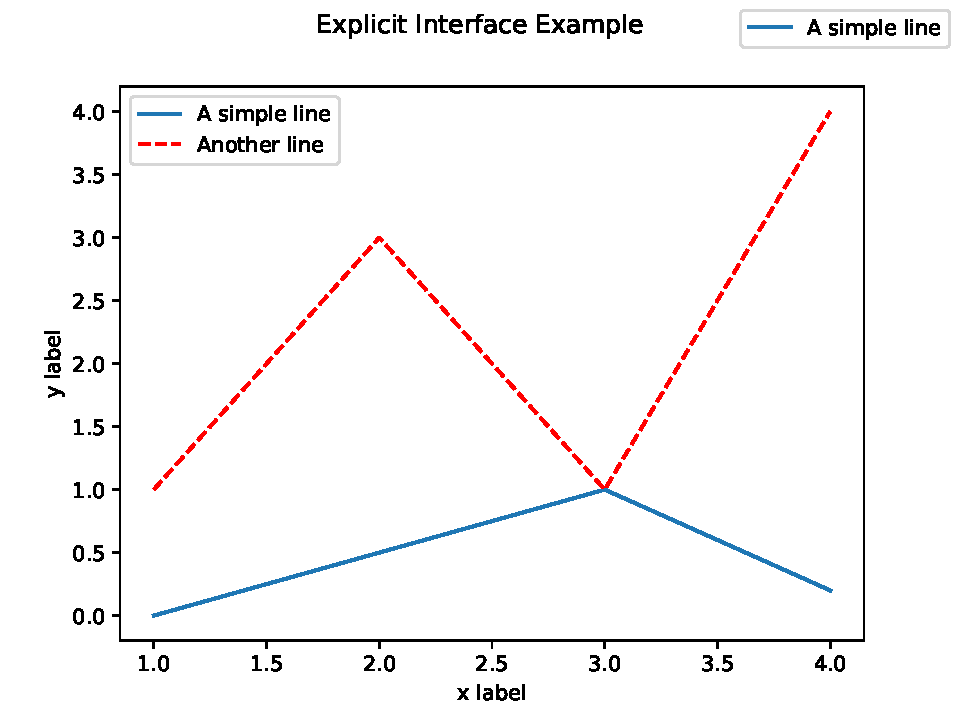
\includegraphics[width=1\textwidth]{/workspaces/python_course/slides/week_five/figures/myplot.pdf}
    \end{figure}
\end{frame}

\section{Debugging}

\begin{frame}{Debugging}
    \begin{itemize}
        \item  <1-> Debugging is the process of finding and fixing errors in your code
        \item  <2-> Special program attached to the running program
        \item <3-> Allows you to inspect the program at runtime
    \end{itemize}
\end{frame}

\begin{frame}{Debugging}
    Usecases:
    \begin{itemize}
        \item cath errors and show you the code and the state of the code
        \item set breakpoints and hold the program at a certain point
    \end{itemize}
\end{frame}

\begin{frame}{Debugging - HowTo}
    \begin{figure}
        \centering
        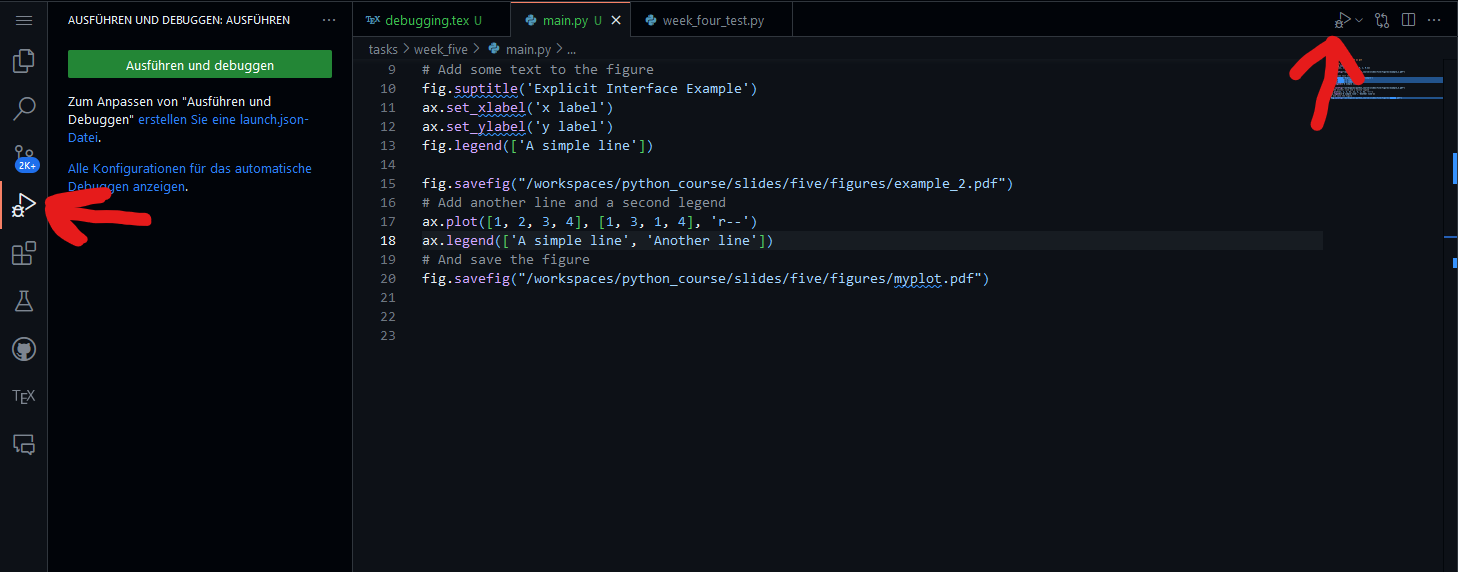
\includegraphics[width=1\textwidth]{/workspaces/python_course/slides/week_five/figures/Screenshot 2023-11-27 163952.png}
    \end{figure}
\end{frame}

\begin{frame}{Debugging - HowTo}
    \begin{figure}
        \centering
        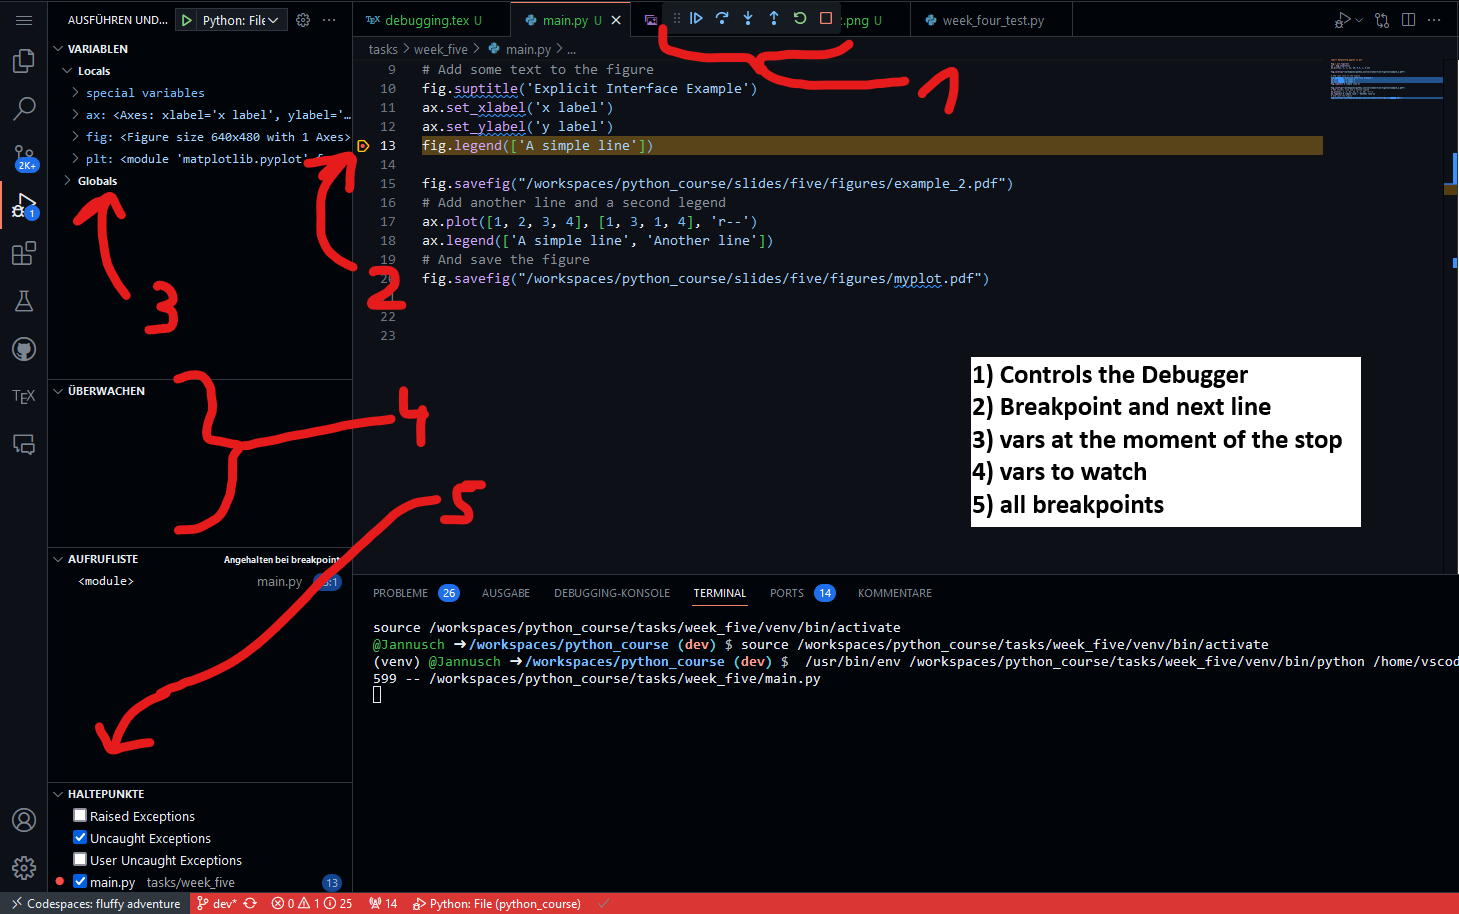
\includegraphics[width=1\textwidth]{/workspaces/python_course/slides/week_five/figures/Screenshot 2023-11-27 165218.png}
    \end{figure}
\end{frame}


\section{Debugging - Example}

\section{Task}

\begin{frame}{Task}
    \begin{itemize}
        \item  Advent of Code again (now with debugger)
        \item  Try to plot some of the data
    \end{itemize}
    
\end{frame}

\begin{frame}[fragile]{Task - Matplotlib}
    \textbf{1. Rebuilt the container}\\
    \textbf{2. Create the environment}
    \begin{lstlisting}[language=bash, backgroundcolor = \color{lightgray}, columns=fullflexible,
        breaklines=true]
    $ cd /workspaces/python_course/tasks/week_five
    $ python3 -m venv venv
    $ source venv/bin/activate
    \end{lstlisting}
    \textbf{3. Install the requirements}
    \begin{lstlisting}[language=bash, backgroundcolor = \color{lightgray}, columns=fullflexible,
        breaklines=true]
    $ pip install matplotlib
    \end{lstlisting}
    \textbf{4. Set the interpreter in VSCode}

\end{frame}

\begin{frame}{Task - Rebuilt the container}
    \begin{figure}
        \centering
        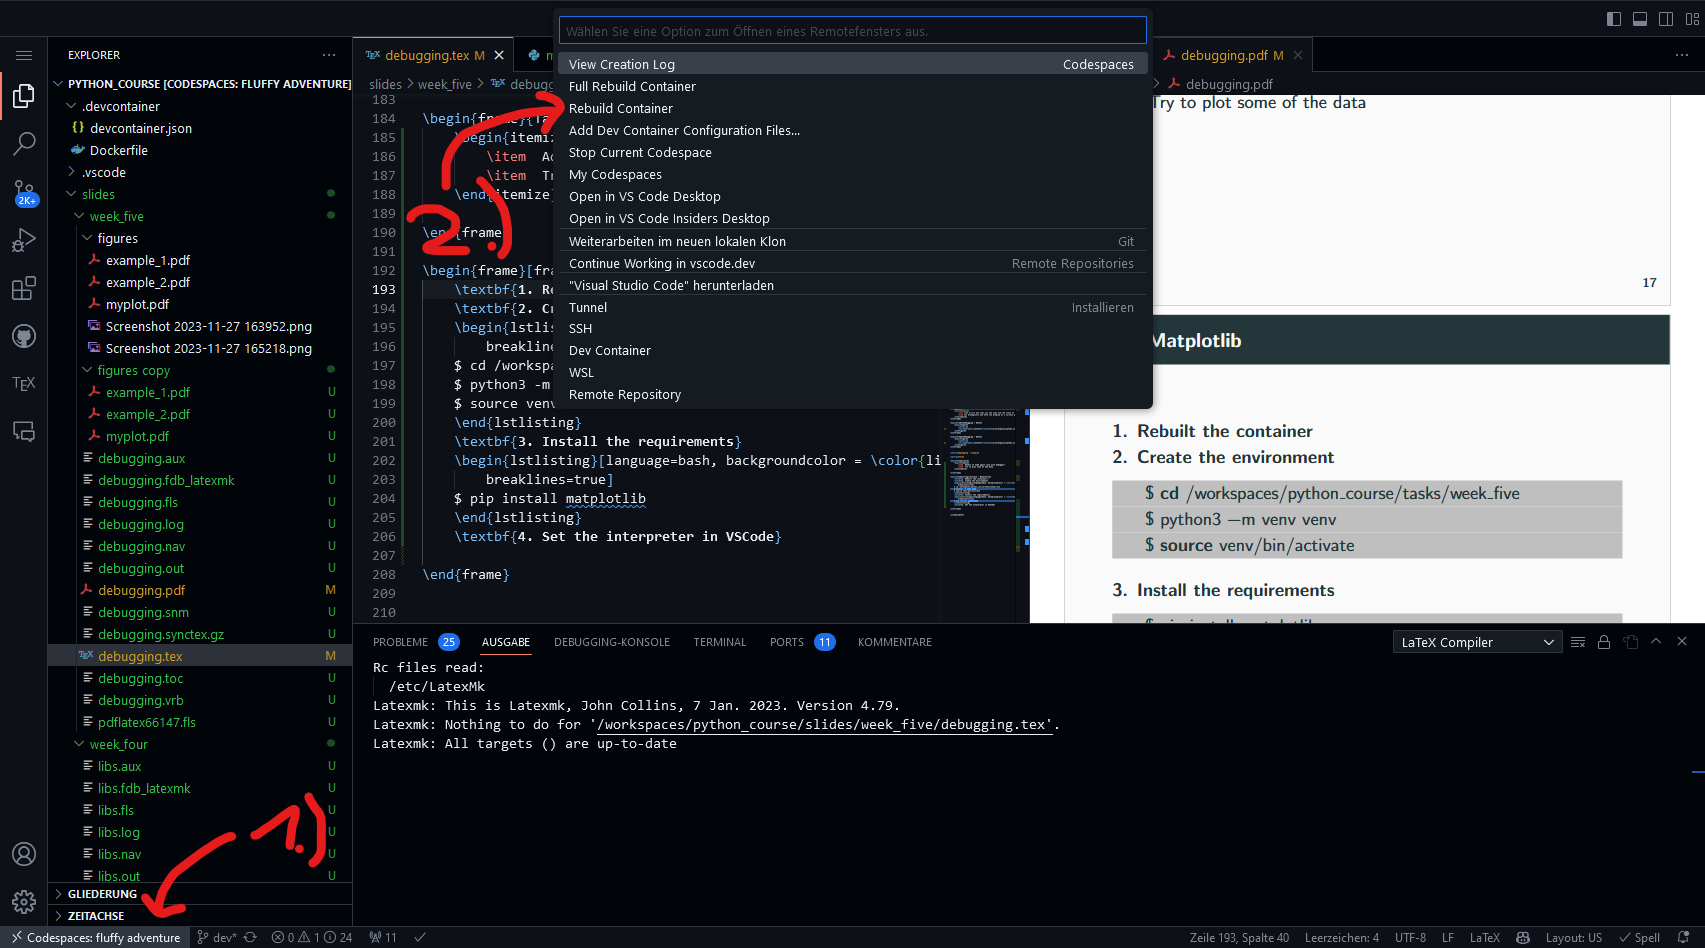
\includegraphics[width=1\textwidth]{/workspaces/python_course/slides/week_five/figures/Screenshot 2023-11-27 180245.png}
    \end{figure}
\end{frame}

\begin{frame}{Task - Set the interpreter}
    \begin{figure}
        \centering
        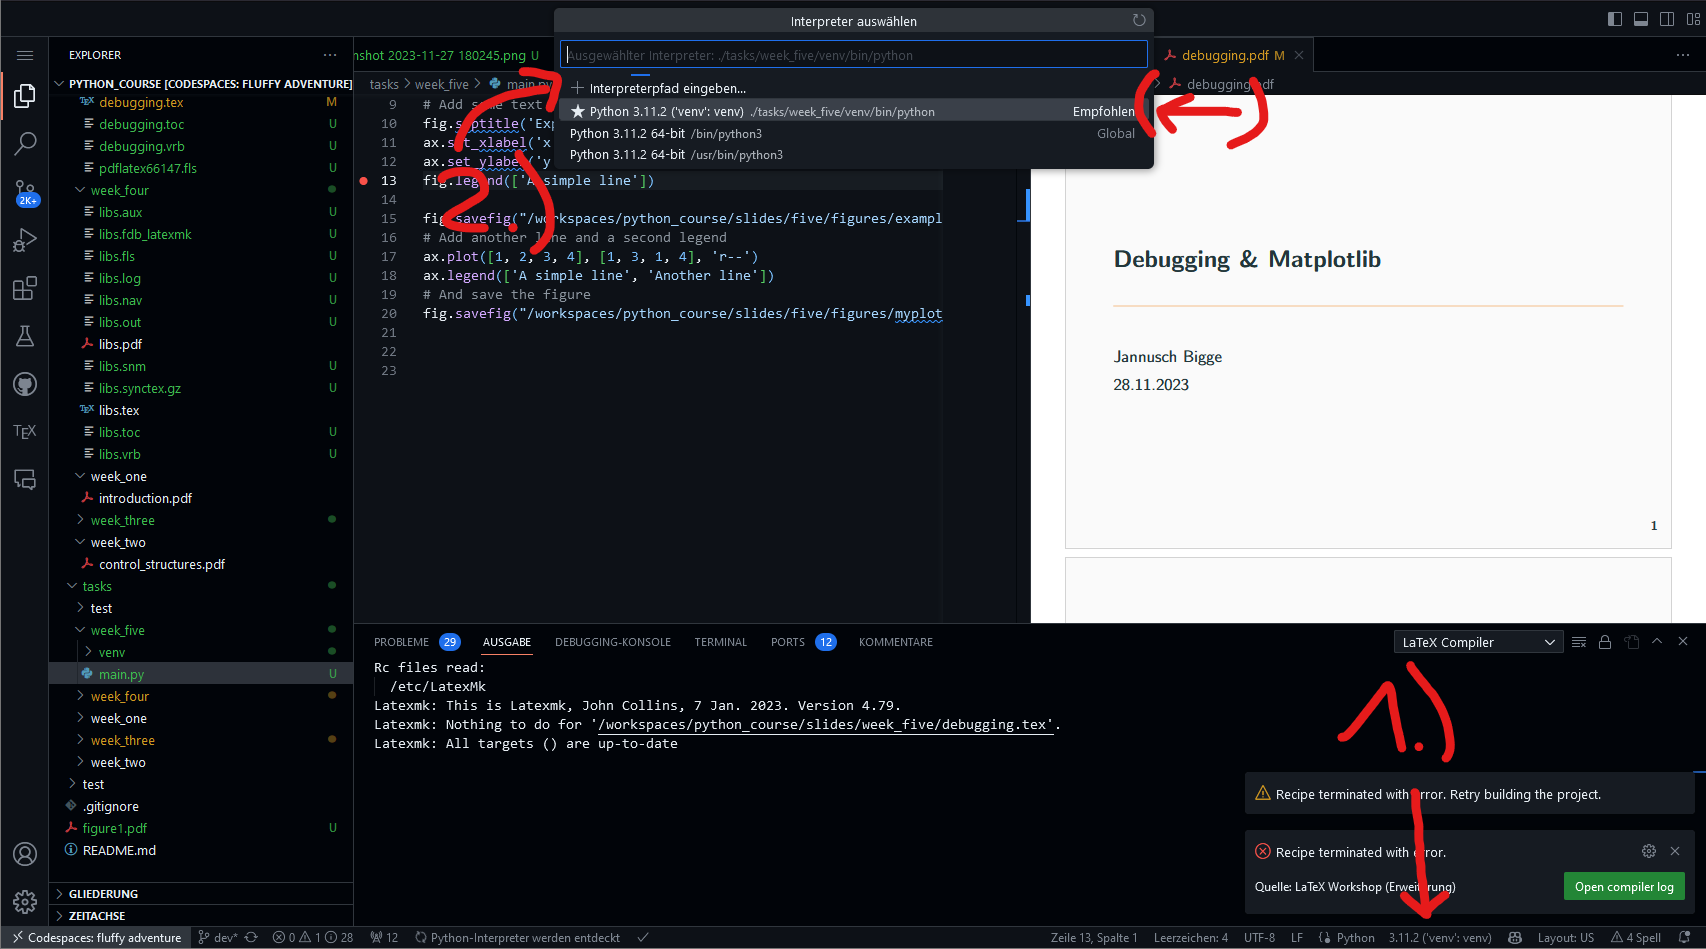
\includegraphics[width=1\textwidth]{/workspaces/python_course/slides/week_five/figures/Screenshot 2023-11-27 180627.png}
    \end{figure}
    Maybe you have to navigate no the path (venv/bin/python). Best case VSCode finds it automatically.
\end{frame}

\end{document}

